\documentclass[a4paper,11pt]{exam}
\printanswers % pour imprimer les réponses (corrigé)
%\noprintanswers % Pour ne pas imprimer les réponses (énoncé)
\addpoints % Pour compter les points
% \noaddpoints % pour ne pas compter les points
%\pointsinmargin
%\qformat{\textbf{\thequestion ) } }
\qformat{\textbf{\thequestion )} (\textit{\thepoints}) \\  }  % Pour définir le style des questions (facultatif)
\usepackage{color} % définit une nouvelle couleur
\shadedsolutions % définit le style des réponses
% \framedsolutions % définit le style des réponses
\definecolor{SolutionColor}{rgb}{0.8,0.9,1} % bleu ciel
\renewcommand{\solutiontitle}{\noindent\textbf{Solution:}\par\noindent} % Définit le titre des solutions

\usepackage{multicol}
\usepackage{caption}
\usepackage{tikz}
\usepackage{tkz-tab}
\usepackage{array}
\usetikzlibrary{trees}
\usepackage[final]{pdfpages}


\makeatletter

\def\maketitle{{\centering%
	\par{\huge\textbf{\@title}}%
	\par{\@date}%
	\par}}


\renewcommand{\thesubsection}{\Alph{subsection}.}   

\makeatother

%\lhead{NOM Pr\'enom :}
%\rhead{\textbf{Les r\'eponses doivent \^etre justifi\'ees et r\'edig\'ees}}
\cfoot{\thepage / \pageref{LastPage}}


%\usepackage{../../pas-math}
%\usepackage{../../moncours}


%\usepackage{pas-cours}
%-------------------------------------------------------------------------------
%          -Packages nécessaires pour écrire en Français et en UTF8-
%-------------------------------------------------------------------------------
\usepackage[utf8]{inputenc}
\usepackage[frenchb]{babel}
\usepackage[T1]{fontenc}
\usepackage{lmodern}
\usepackage{textcomp}



%-------------------------------------------------------------------------------

%-------------------------------------------------------------------------------
%                          -Outils de mise en forme-
%-------------------------------------------------------------------------------
\usepackage{hyperref}
\hypersetup{pdfstartview=XYZ}
%\usepackage{enumerate}
\usepackage{graphicx}
\usepackage{multicol}
\usepackage{tabularx}
\usepackage{multirow}


\usepackage{anysize} %%pour pouvoir mettre les marges qu'on veut
%\marginsize{2.5cm}{2.5cm}{2.5cm}{2.5cm}

\usepackage{indentfirst} %%pour que les premier paragraphes soient aussi indentés
\usepackage{verbatim}
\usepackage{enumitem}
\usepackage[usenames,dvipsnames,svgnames,table]{xcolor}

\usepackage{variations}

%-------------------------------------------------------------------------------


%-------------------------------------------------------------------------------
%                  -Nécessaires pour écrire des mathématiques-
%-------------------------------------------------------------------------------
\usepackage{amsfonts}
\usepackage{amssymb}
\usepackage{amsmath}
\usepackage{amsthm}
\usepackage{tikz}
\usepackage{xlop}
%-------------------------------------------------------------------------------



%-------------------------------------------------------------------------------


%-------------------------------------------------------------------------------
%                    - Mise en forme avancée
%-------------------------------------------------------------------------------

\usepackage{ifthen}
\usepackage{ifmtarg}


\newcommand{\ifTrue}[2]{\ifthenelse{\equal{#1}{true}}{#2}{$\qquad \qquad$}}

%-------------------------------------------------------------------------------

%-------------------------------------------------------------------------------
%                     -Mise en forme d'exercices-
%-------------------------------------------------------------------------------
%\newtheoremstyle{exostyle}
%{\topsep}% espace avant
%{\topsep}% espace apres
%{}% Police utilisee par le style de thm
%{}% Indentation (vide = aucune, \parindent = indentation paragraphe)
%{\bfseries}% Police du titre de thm
%{.}% Signe de ponctuation apres le titre du thm
%{ }% Espace apres le titre du thm (\newline = linebreak)
%{\thmname{#1}\thmnumber{ #2}\thmnote{. \normalfont{\textit{#3}}}}% composants du titre du thm : \thmname = nom du thm, \thmnumber = numéro du thm, \thmnote = sous-titre du thm

%\theoremstyle{exostyle}
%\newtheorem{exercice}{Exercice}
%
%\newenvironment{questions}{
%\begin{enumerate}[\hspace{12pt}\bfseries\itshape a.]}{\end{enumerate}
%} %mettre un 1 à la place du a si on veut des numéros au lieu de lettres pour les questions 
%-------------------------------------------------------------------------------

%-------------------------------------------------------------------------------
%                    - Mise en forme de tableaux -
%-------------------------------------------------------------------------------

\renewcommand{\arraystretch}{1.7}

\setlength{\tabcolsep}{1.2cm}

%-------------------------------------------------------------------------------



%-------------------------------------------------------------------------------
%                    - Racourcis d'écriture -
%-------------------------------------------------------------------------------

% Angles orientés (couples de vecteurs)
\newcommand{\aopp}[2]{(\vec{#1}, \vec{#2})} %Les deuc vecteurs sont positifs
\newcommand{\aopn}[2]{(\vec{#1}, -\vec{#2})} %Le second vecteur est négatif
\newcommand{\aonp}[2]{(-\vec{#1}, \vec{#2})} %Le premier vecteur est négatif
\newcommand{\aonn}[2]{(-\vec{#1}, -\vec{#2})} %Les deux vecteurs sont négatifs

%Ensembles mathématiques
\newcommand{\naturels}{\mathbb{N}} %Nombres naturels
\newcommand{\relatifs}{\mathbb{Z}} %Nombres relatifs
\newcommand{\rationnels}{\mathbb{Q}} %Nombres rationnels
\newcommand{\reels}{\mathbb{R}} %Nombres réels
\newcommand{\complexes}{\mathbb{C}} %Nombres complexes


%Intégration des parenthèses aux cosinus
\newcommand{\cosP}[1]{\cos\left(#1\right)}
\newcommand{\sinP}[1]{\sin\left(#1\right)}


%Probas stats
\newcommand{\stat}{statistique}
\newcommand{\stats}{statistiques}
%-------------------------------------------------------------------------------

%-------------------------------------------------------------------------------
%                    - Mise en page -
%-------------------------------------------------------------------------------

\newcommand{\twoCol}[1]{\begin{multicols}{2}#1\end{multicols}}


\setenumerate[1]{font=\bfseries,label=\textit{\alph*})}
\setenumerate[2]{font=\bfseries,label=\arabic*)}


%-------------------------------------------------------------------------------
%                    - Elements cours -
%-------------------------------------------------------------------------------





%\usepackage{fullpage}
\author{\ }
\date{24 Décembre 2017}
\title{Terminale ST$_2$S : DS num\'ero 2}


\begin{document}
%	\usepackage{fancyhdr}
%	
%	\pagestyle{fancy}
%	\fancyhf{}
	%\rhead{Share\LaTeX}

	%\maketitle
	
	\begin{center}
	%\centering
	
	{\scshape\LARGE \textbf{BACCALAUR\'EAT TECHNOLOGIQUE} \par}
	\vspace{1cm}
	{\scshape\Large \textbf{SESSION 2018}\par}
	\vspace{1.5cm}
	

	\begin{large}
		\begin{tabular}{|@{\ }c@{\ }|@{\ }c@{\ }|}
		\hline
		%\ & \ \\
		\'Epreuve : \textbf{MATH\'EMATIQUES} & Série : \textbf{Sciences et Technologies de}  \\ 
		\textit{\'Epreuve blanche}&  \textbf{la Santé et du Social (ST2S)} \\ \hline
		\ & \ \\
		Durée de l'épreuve : \textbf{2 heures} & Coefficient : \textbf{3} \\ 
		\ & \ \\
		\hline
	\end{tabular}
	\end{large}
		
	\vspace{1cm}
	{\large\bfseries \'EPREUVE DU MERCREDI 26 AVRIL 2018}
	
	\vspace{1cm}
	{\itshape L'usage d'une calculatrice autorisé selon la réglementation en vigueur\par}
	%\vfill
	\vspace{1.5cm}
	{\bfseries Ce sujet comporte \pageref{LastPage} pages numérotées de 1/\pageref{LastPage} à \pageref{LastPage}/\pageref{LastPage} }
	
%	\vspace{0.5cm}
%	{\bfseries Ce sujet comporte x annexes situés pages \pageref{annexe} /\pageref{LastPage} à \pageref{LastPage}/\pageref{LastPage} à remettre avec la copie.}
	
	\vspace{0.5cm}
	{\bfseries\itshape Le candidat doit s'assurer que le sujet distribué est complet. }
	
	\vfill	
	
	\fbox{
		\begin{minipage}{0.9\textwidth}
			\large
			Il  est  rappelé  que  la  qualité  de  la  rédaction,  la  clarté  et  la  précision  des  raisonnements entreront pour une part importante dans l'appréciation des copies. 
			
			Cependant, le candidat est invité à faire figurer sur la copie toute trace de recherche, même incomplète ou infructueuse, qu'il aura développée. 
		\end{minipage}
	}
	
	\vfill

% Bottom of the page
	%{\large \today\par}
\end{center}
\newpage

\ 
\ 
\\

\newpage



\section{Lectrure des propriétés d'une fonction à partir d'un tableau de variation}

On donne ci-dessous les variations d'une fonction $f$, définie et dérivable sur $[-10;20]$, et on nomme $\mathcal{C}$ sa représentation graphique dans un repère orthonormal $(O, \vec{i}, \vec{j})$ :

Répondre par $VRAI$ ou $FAUX$, aux questions suivantes (une justification est demandée lorsque la réponse est $FAUX$, aucune justification n'est demandée lorsque la réponse est $VRAI$).

\begin{center}
	\begin{tikzpicture}[scale=0.8]
		\tkzTabInit{$x$/1.5,$f(x)$/4}{$-10$, $0$, $4$, $9$, $20$}
		%\tkzTabLine { ,+ ,z , -, }
		\tkzTabVar{+/$10$,-/$-2$,+/$3$,-/$-1$,+/$0$}
	\end{tikzpicture}
\end{center}

\begin{questions}
	\question[1]  Pour tout réel $x$, $f(x) \ge -2$.
	\question[1]  L'équation $f(x)=-3$ admet au moins une solution dans $[-10;20]$.
	\question[1] L'équation $f(x)=1$ admet une solution unique dans $[4;9]$.
	\question[1] Pour tout réel $x$, $f'(x)\ge 0$.
	\question[1] $f'(1)<0$.
\end{questions}


\newpage

\section{(6 points)}

Le tableau suivant, extrait d'une feuille d'un tableur, donne le prix annuel moyen du paquet de cigarettes (20 cigarettes) le plus vendu, en euros, entre 2000 et 2004.

\begin{center}
	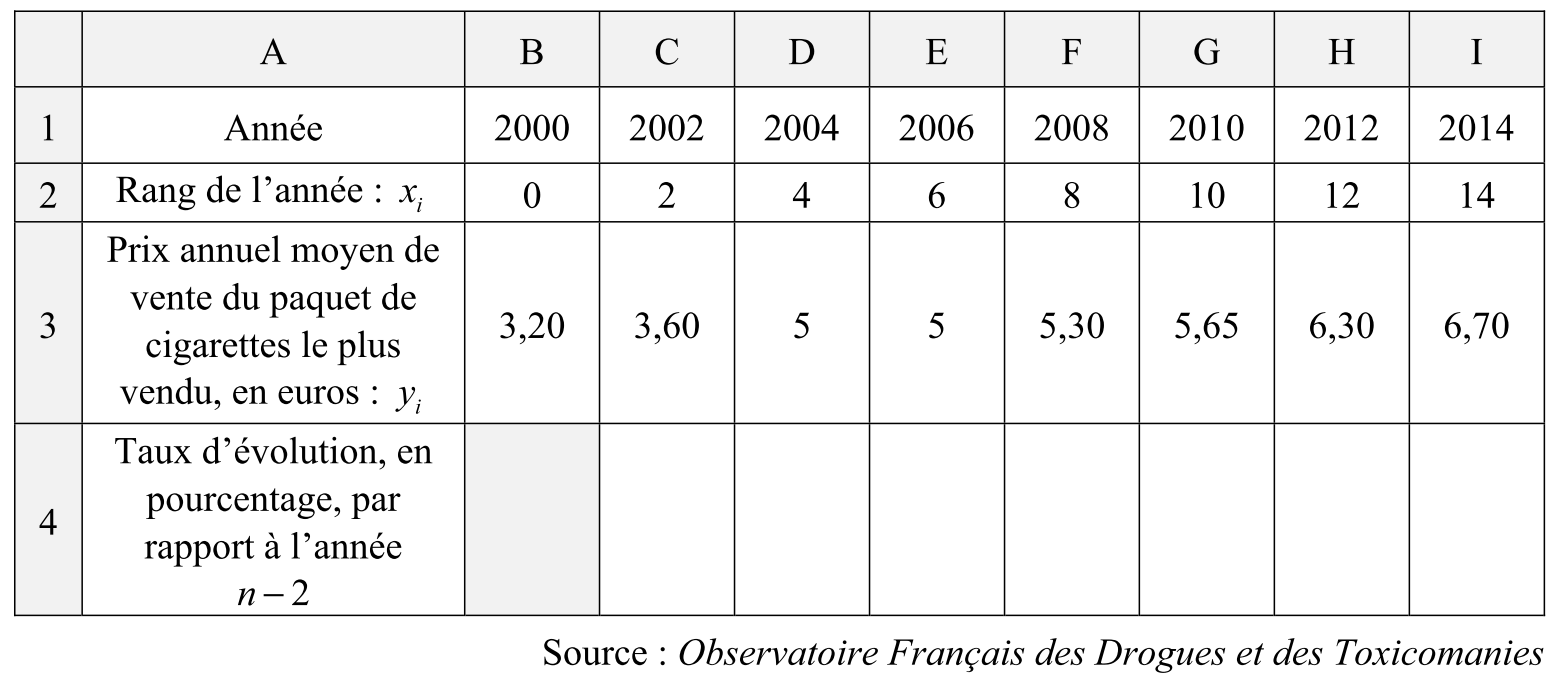
\includegraphics[scale=0.4]{img/tabac}
\end{center}

\subsection{(2 points)}

\begin{questions}
	\question[1] Un journaliste affirme que le prix entre 2000 et 2014 a augmenté de $50$ \%. L'affirmation est-elle vraie ou fausse ? Justifier.
	
	\question[1] La ligne 4 est au format pourcentage. Quelle formule peut-on saisir dans la cellule $C4$ et recopier vers la droite pour compléter la ligne 4 ?
\end{questions}

\subsection{(4 points)}

\begin{questions}
	\question[2]
	
		\begin{parts}
			\part[1] Sur la feuille de papier millimétré fournie et à rendre avec la copie, représenter le nuage de points de coordonnées $(x_i;y_i)$ dans un repère orthogonal en choisissant :
			\begin{itemize}
				\item 1cm pour 2 années en abscisse ;
				\item 1cm pour 1 euro en ordonnée.
			\end{itemize}
		
			\part[1] Calculer les coordonnées du point moyen $G$ du nuage de points, puis placer le point $G$ sur le graphique précédent. Arrondir les résultats à \num{0.01} près.
		\end{parts}
	
	\question[2] On admet que la droite $D$ d'équation $y=\num{0.24}x+\num{3.41}$ est un bon ajustement affine du nuage de points et que cet ajustement reste valable jusqu'en 2025.
		\begin{parts}
			\part[\half] Vérifier que le point $G$ appartient à la droite $D$.
			\part[\half] Tracer la droite $D$ sur le graphique précédent en indiquant les points utilisés.
			\part[\half] Selon cet ajustement, quel sera le prix moyen annuel d'un paquet de cigarettes en France en 2020 ?
			\part[\half] \'A partir de quelle année celui-ci dépassera-t-il les 10 euros ? Expliquer la démarche.
		\end{parts}
\end{questions}
%
\newpage
%	
\section{(9 points)}

\subsection{(4 points)}

Entre le $1^{er}$ janvier 2014 et le 31 décembre 2014, une clinique enregistre \num{1200} accouchements. Depuis quelques années, le nombre annuel d'accouchements a augmenté de 3 \% par an. L'objectif du directeur de la clinique est d'atteindre les \num{8000} accouchements réalisés dans la clinique d'ici fin 2020, en supposant que ce pourcentage d'augmentation moyen reste constant.\\

Pour tout nombre entier naturel $n$, on note $u_n$ le nombre annuel d'accouchements dans cette clinique pour l'année $2014+n$. Ainsi $u_0$ est le nombre d'accouchements durant l'année 2014, et $u_0=\num{1200}$.

\begin{questions}
	\question[\half] Déterminer le nombre d'accouchements  qui ont eu lieu dans cette clinique en 2015.
	\begin{solution}
		Le coefficient multiplicateur correspondant à une augmentetion de 3\% est \num{1.03}.
		
		$1200 \times \num{1.03} = 1236$
		
		En 2015, il y a eu \num{1236} accouchements dans cette clinique.
	\end{solution}
	\question[1] Quelle est la nature de la suite $(u_n)$ ? Justifier et donner ses éléments caractéristiques.
	\begin{solution}
		Chaque année, le nombre de naissance augmente de 3\%, donc chaque terme de la suite est obtenu en multipliant le précédent par \num{1.03}. C'est une suite géométrique de terme initial $u_0 = 1200$ et de raison $q=\num{1.03}$.
	\end{solution}
	\question[1] Pour tout entier naturel $n$, exprimer $u_n$ en fonction de $n$.
	\begin{solution}
		Expression de $u_n$ en fonction de $n$ :
		
		\begin{eqnarray*}
			u_n &=& u_0 \times q^n \\
			u_n &=& \num{1200} \times \num{1.03}^n 
		\end{eqnarray*}
	\end{solution}

	\question[\half] Déterminer le nombre d'accouchements qui auront lieu dans cette clinique en 2017 selon ce modèle. On arrondira ce résultat à l'unité.
	\begin{solution}
		$2017 - 2014 = 3$, calcul de $u_3$ :
		
		\begin{eqnarray*}
			u_3 &=& \num{1200} \times \num{1.03}^3 \\
			u_3 & \approx & \num{1311}
		\end{eqnarray*}
	
	En 2017, il y aura \num{1311} accouchements.
	\end{solution}
	\question[1] On rappelle le résultat suivant :
	
	Si $(u_n)$ est une suite géométrique de premier terme $u_0$ et de raison $q$, $q\neq1$, alors :
	\begin{equation*}
		u_0 + u_1 + u_2 + ... + u_n = u_o \times \dfrac{1-q^{n+1}}{1-q}
	\end{equation*}

	\begin{parts}
		\part[] Déterminer le nombre total d'accouchements qui auront lieu dans cette clinique entre le $1^{er}$ janvier 2014 et el 31 décembre 2020. On arrondira le résultat à l'unité.
		\begin{solution}
			
			2020 est l'année de rang 6, calcul de $S_{20}$:
			\begin{eqnarray*}
				S_{20} &=& 1200 \times \dfrac{1 - \num{1.03}^7}{1 - 1\num{1.03}} \\
				S_{20} & \approx & \num{9195}
			\end{eqnarray*}
		
		Selon ce modèle, il y aura \num{9195} accouchements dans cette clinique entre 2014 et 2020.
		\end{solution}
		\part[] Selon ce modèle, le directeur peut-il espérer atteindre son objectif ? Justifier.
		\begin{solution}
			9195 est supérieur à 8000, donc le directeur peut atteindre son objectif.
		\end{solution}
		
	\end{parts}
\end{questions}

\subsection{(5 points)}

L'Organisation Mondiale de la Santé (OMS) recommande un taux maximum de 15 \% de césariennes pour ce type de clinique. En France, les experts estiment que le taux de césariennes est anormal s'il dépasse les 25 \%.\\

Un journal régional a mené une enquête auprès d'un certain nombre de femmes ayant accouché dans la clinique en 2014. L'objectif de cette étude était de déterminer si la clinique avait tendance à recourir trop fréquemment à une césarienne sans réelle justification médicale. Lors de cette enquête, le journaliste a obtenu les résultats suivants :

\begin{itemize}
	\item 43 \% des femmes interrogées sont primipares (c'est-à-dire qu'il s'agit de leur premier enfant) et parmi elles, 23 \% ont accouché par césarienne à la clinique.
	\item 11 \% des femmes interrogées sont des multipares (c'est-à-dire qu'elles ont déjà accouché auparavant) ayant accouché par césarienne lors d'un accouchement précédent et parmi elles, 64 \% ont accouché par césarienne à la clinique.
	\item Les autres sont de multipares n'ayant jamais accouché par césarienne auparavant et parmi elles, 8 \% ont accouché par césarienne à la clinique.	
\end{itemize}

On choisit au hasard une femme ayant participé à l'enquête.
On considère les événements suivants :
\begin{itemize}
	\item[$A_0$ :]  <<La femme est une primipare >> (c'est-à-dire qu'il s'agit de son premier enfant);
	\item[$M_1$ :]  <<La femme est une multipare qui a déjà accouché par césarienne >> ;
	\item[$M_2$ :]  <<La femme est une multipare qui n'a jamais accouché par césarienne auparavant>> ;
	\item[$C$ :] <<La femme a accouché par césarienne à la clinique>>.
\end{itemize}

L'événement contraire de l'événement $C$ est noté $\bar{C}$.

\begin{questions}
	\question[1] \'A partir des données de l'énoncé, déterminer :
		\begin{parts}
			\part[\half] La probabilité de l'événement $M_1$, notée $P(M_1)$;
			\begin{solution}
				$P(M_1) = \frac{11}{100} = \num{0.11}$
			\end{solution}
			\part[\half] La probabilité que la femme ait accouché par césarienne sachant qu'elle est une multipare qui a déjà accouché par césarienne, notée $P_{M_1}(C)$.
			\begin{solution}
				$P_{M_1}(C) = \frac{64}{100} = \num{0.64}$
			\end{solution}
		\end{parts}
	
	\question[1] Recopier et compléter l'arbre ci-dessous :
	
	\input{tree3}
	
	\begin{solution}
			
% Set the overall layout of the tree
\tikzstyle{level 1}=[level distance=3.5cm, sibling distance=3.5cm]
\tikzstyle{level 2}=[level distance=3.5cm, sibling distance=2cm]

% Define styles for bags and leafs
\tikzstyle{bag} = [text width=4em, text centered]
\tikzstyle{end} = [circle, minimum width=3pt,fill, inner sep=0pt]

% The sloped option gives rotated edge labels. Personally
% I find sloped labels a bit difficult to read. Remove the sloped options
% to get horizontal labels. 
\begin{tikzpicture}[grow=right, sloped]
\node[bag] {}
    child {
        node[bag] {$M_2$}        
            child {
                node[end, label=right:
                    {$\bar{C}$ }] {}
                edge from parent
                node[below] {$0,92$}
                %node[below]  {$\frac{4}{9}$}
            }
            child {
                node[end, label=right:
                    {$C$}] {}
                edge from parent
                node[above] {$0,08$}
                %node[below]  {$\frac{5}{9}$}
            }
            edge from parent 
            %node[above] {$W$}
            node[below]  {$0,46$}
    }
    child {
        node[bag] {$M_1$}        
        child {
                node[end, label=right:
                    {$\bar{C} $}] {}
                edge from parent
                %node[above] {$B$}
                node[below]  {$0,36$}
            }
            child {
                node[end, label=right:
                    {$C$}] {}
                edge from parent
                node[above] {$0,64$}
%                node[below]  {$\frac{6}{9}$}
            }
        edge from parent         
            %node[above] {$B$}
            node[above]  {$0,11$}
    }
    child {
    	node[bag] {$A_0$}        
    	child {
    		node[end, label=right:
    		{$\bar{C}$}] {}
    		edge from parent
    		%node[above] {$B$}
    		node[below]  {$0,77$}
    	}
    	child {
    		node[end, label=right:
    		{$C$}] {}
    		edge from parent
    		node[above] {$0,23$}
    		%                node[below]  {$\frac{6}{9}$}
    	}
    	edge from parent         
    	%node[above] {$B$}
    	node[above]  {$0,43$}
    };
\end{tikzpicture}

	\end{solution}
%		\begin{center}
%			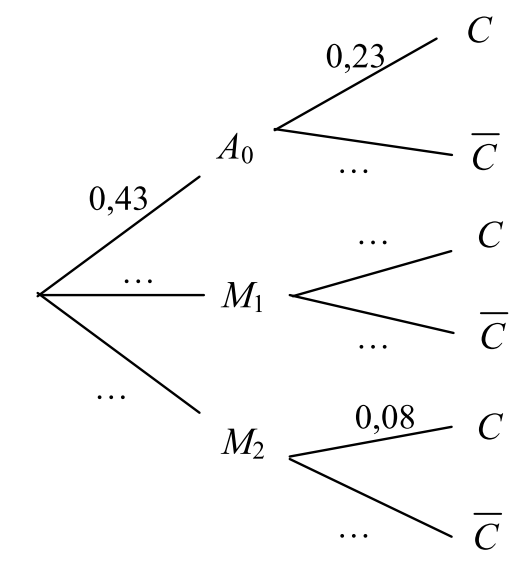
\includegraphics[scale=0.4]{img/arbre}
%		\end{center}	
	
	\question[1] Définir par une phrase l'événement $A_0 \cap C$ puis calculer la probabilité $P(A_0 \cap C)$.
	\begin{solution}
		$A_0 \cap C$ : <<La femme est une primipare et elle a accouché par césarienne à la clinique.>>
		
		\begin{eqnarray*}
			P(A_0 \cap C) &=& \num{0.43} \times \num{0.23} \\
			P(A_0 \cap C) &=& \num{0.0989}
		\end{eqnarray*}
	\end{solution}
	
	\question[1] Montrer que la probabilité qu'une femme accouche par césarienne dans cette clinique est égale à \num{0.2061}.
	\begin{solution}
		Calcul de $P(M_1 \cap C)$ et $P(M_2 \cap C)$.
		
		\begin{eqnarray*}
			P(M_1 \cap C) &=& \num{0.11} \times \num{0.64} \\
			P(M_1 \cap C) &=& \num{0.0704} \\
			& & \\
			P(M_2 \cap C) &=& \num{0.08} \times \num{0.23} \\
			P(M_2 \cap C) &=& \num{0.0368} 			
		\end{eqnarray*}
	
	Calcul de $P(C)$ :
	\begin{eqnarray*}
		P(C) &=& P(A_0 \cap C) + P(M_1 \cap C) + P(M_2 \cap C) \\
		P(C) &=& \num{0.0989} + \num{0.0704} + \num{0.0368} \\
		P(C) &=& 0.2061				
	\end{eqnarray*}
	\end{solution}
	
	\question[1] La clinique étudiée respecte-t-elle les recommandations de l'OMS ? Des experts français ?
	\begin{solution}
		Dans cette clinique, le taux de césarienne est de \num{20.61} \%, donc elle respecte les recommandations des experts français mais pas celles de l'OMS. 
	\end{solution}
		
\end{questions}
%
%\appendix


	\label{LastPage}

\newpage
%\thispagestyle{empty}

\includepdf[pages={2}]{essai}
%\thispagestyle{empty}
\centering
\begin{tikzpicture}
	% Dimensions du repere
	\def\xmin{0} \def\xmax{19} \def\ymin{0} \def\ymax{28}
	% Grilles
	\draw [step=0.1cm,gray,ultra thin]  (\xmin,\ymin) grid (\xmax,\ymax);
	\draw [step=0.5cm,gray, thin] (\xmin,\ymin) grid (\xmax,\ymax);
	\draw [step=1cm,gray, thick] (\xmin,\ymin) grid (\xmax,\ymax);
	\draw [step=5cm,gray,very thick] (\xmin,\ymin) grid (\xmax,\ymax);

	%\draw [step=0.25cm,gray,very thin] (\xmin,\ymin) grid (\xmax,\ymax);
	%\draw [step=1cm,gray,thin] (\xmin,\ymin) grid (\xmax,\ymax);
	%\draw [step=5cm,thick,color=black]  (\xmin,\ymin) grid (\xmax,\ymax); 	
\end{tikzpicture}

%\label{annexe}

	

\end{document}